\documentclass{beamer}
\usetheme{Boadilla}

\usepackage{amsmath}
\usepackage{amsfonts}
\usepackage{hyperref}
\usepackage{amsthm}
\usepackage{algorithm}
\usepackage{algpseudocode}



\title{Knowledge Transfer via Dense Cross-Layer
Mutual-Distillation}
\author{Skorik Sergey}
\institute{MIPT, 2023}


\begin{document}

\begin{frame}
    \titlepage
\end{frame}


\begin{frame}
    \tableofcontents
\end{frame}

\section{Method}

\begin{frame}{Knowledge distillation}
    \begin{block}{Formulation}
        Review the formulation of Knowledge Distillation (KD). \\
        Given the training data $X=\{x_n\}_{n=1}^N$ and , the ground-truth labels are denoted as $Y = \{y_n\}_{n=1}^N$. Let $W_t$ be a teacher network trained beforehand and fixed, and let $W_s$ be a student model. In KD, the student network $W_s$ is trained by minimizing
        \begin{equation}\label{KD_objective}
            L_s = L_c(W_s, X, Y) + \lambda L_{kd}(\hat{P}_t, \hat{P}_s)
        \end{equation}
        Where $L_c$ classification loss by hard labels, $L_{kd}$ is the distillation loss
        \begin{equation}\label{KD_distill_loss}
            L_{kd}(\hat{P}_t, \hat{P}_s) = -\dfrac{1}{N}\sum_{n=1}^N\sum_{m=1}^M\hat{P}_t^m(x_n) \log \hat{P}_s^m(x_n)
        \end{equation}
    \end{block}
\end{frame}

\begin{frame}{Deep Mutual Learning}
    \begin{block}{Formulation}
        DML can be viewed as a bidirectional KD method that jointly trains the teacher and student networks via interleavingly optimizing two objectives:
        \begin{equation}\label{DML_onjective}
        \begin{split}
            L_s = L_c(W_s, X, Y) + \lambda L_{dml}(\hat{P}_t, \hat{P}_s) \\
            L_t = L_c(W_t, X, Y) + \lambda L_{dml}(\hat{P}_s, \hat{P}_t)
        \end{split}
        \end{equation}
         instead of using \eqref{KD_distill_loss}, DML uses Kullback-Leibler divergence:
         \begin{equation}\label{DML_distill_loss}
             L_{dml}(\hat{P}_t, \hat{P}_s) = \dfrac{1}{N}\sum_{n=1}^N\sum_{m=1}^M\hat{P}_t^m(x_n) \log \dfrac{\hat{P}_t^m(x_n)}{\hat{P}_s^m(x_n)}
         \end{equation}
    \end{block}
\end{frame}

\begin{frame}{Dense Cross-Layer Mutual-Distillation}
    \begin{block}{Formulation}
        Let $Q = \{(t_k, s_k)\}_{k=1}^K$ be a set containing $K$ pairs of the same-staged layer indices of the teacher network $W_t$ and the student network $W_s$, indicating the locations where auxiliary classifiers are added. Let $(t_{K+1}, s_{K+1})$ indicating the head classifiers. DCM simultaneously minimizes the following two objectives:
        \begin{equation}\label{DCM_objective}
        \begin{split}
            L_s = L_c(W_s, X, Y) + \alpha L_{ds}(W_s, X, Y) + \beta L_{dcm_1}(\hat{P}_t, \hat{P}_s) + \gamma L_{dcm_2}(\hat{P}_t, \hat{P}_s)\\
            L_t = L_c(W_t, X, Y) + \alpha L_{ds}(W_t, X, Y) + \beta L_{dcm_1}(\hat{P}_s, \hat{P}_t) + \gamma L_{dcm_2}(\hat{P}_s, \hat{P}_t)
        \end{split}
        \end{equation}
    \end{block}
\end{frame}

\begin{frame}{Dense Cross-Layer Mutual-Distillation}
    \begin{block}{Formulation}
        $L_{ds}$ denotes the total cross-entropy loss over all auxiliary classifiers added to the different-staged layers of the student network, which is computed as
        \begin{equation}\label{DCM_distillation}
            L_{ds}(W_s, X, Y) = \sum_{k=1}^K L_c(W_{s_k}, X, Y)
        \end{equation}
        $L_{dcm_1}$, $L_{dcm_2}$ denotes the total loss of the same-staged and different-staged bidirectional KD operations respectevily, which is defined as
        \begin{equation}\label{DCM_same_staged_loss}
            L_{dcm_1}(\hat{P}_t, \hat{P}_s) = \sum_{k=1}^K L_{kd}(\hat{P}_{t_k}, \hat{P}_{s_k})
        \end{equation}
        \begin{equation}\label{DCM_diff_staged_loss}
            L_{dcm_2}(\hat{P}_t, \hat{P}_s) = \sum_{\{(i, j) : 1 \leqslant i, j \leqslant K + 1, i \neq j\}} L_{kd}(\hat{P}_{t_i}, \hat{P}_{s_j})
        \end{equation}
    \end{block}
\end{frame}

\begin{frame}{Dense Cross-Layer Mutual-Distillation}
    \begin{figure}
        \centering
        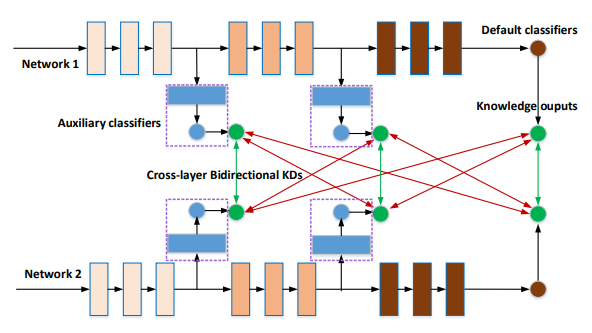
\includegraphics[scale=0.4]{overview.png}
        \caption{Structure overview of the proposed method.}
        \label{fig:overview}
    \end{figure}
\end{frame}

\begin{frame}{Dense Cross-Layer Mutual-Distillation}
    \begin{figure}
        \centering
        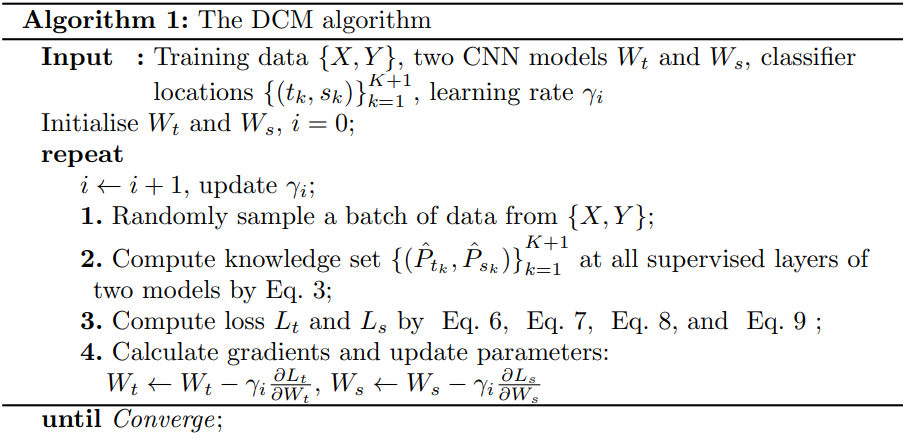
\includegraphics[scale=0.3]{algorithm.png}
        \label{fig:alg}
    \end{figure}
\end{frame}

\section{Experiments}

\begin{frame}{Experiments on CIFAR-100}
    \begin{figure}
        \centering
        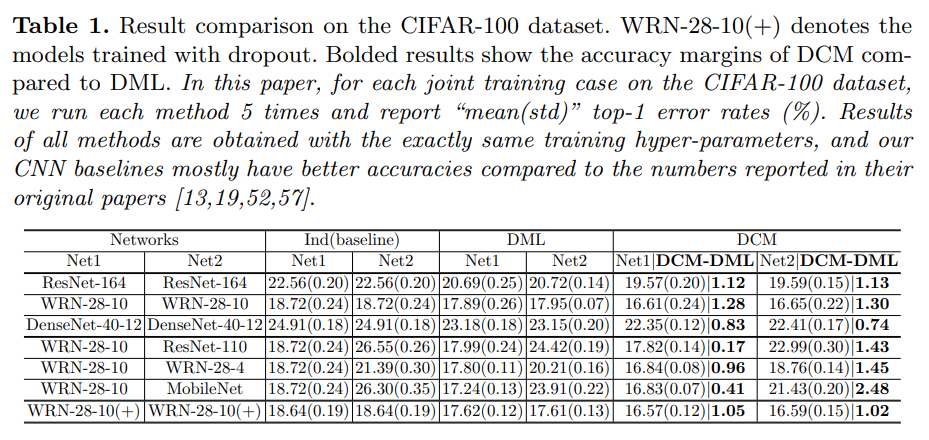
\includegraphics[scale=0.35]{CIFAR100_res.png}
        \label{fig:CIFAR_100_res}
    \end{figure}
\end{frame}

\begin{frame}{Experiments on ImageNet}
    \begin{figure}
        \centering
        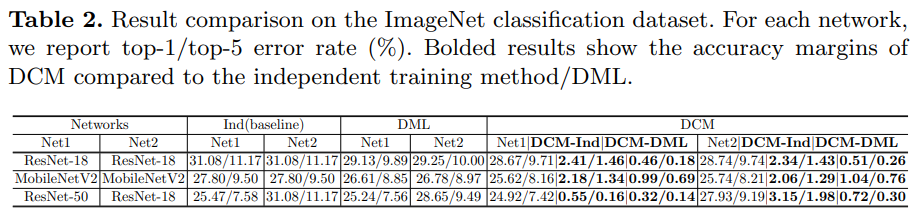
\includegraphics[scale=0.35]{ImageNet_res.png}
        \label{fig:ImageNet_res}
    \end{figure}
\end{frame}

\begin{frame}{Deep Analysis of DCM}
    \begin{block}{Summary}
        \begin{itemize}
            \item Variation of the location and structure of auxiliary classifiers can give an improvement (specifying the $Q$ set)
            \item $L_{dcm_2}$ loss term gives more impact on accuracy. 
            \item A simple addition of classifiers to the DML without using the objective terms $L_{dcm_1}$, $L_{dcm_2}$ or to the baseline method with their independent training does not bring a significant improvement. Thus, the improvement of DCM in comparison with other methods is directly related to the learning mechanism, and not due to an increase in the number of neural network parameters. 
        \end{itemize}
    \end{block}
\end{frame}
\end{document}
